% ============================================================================
% Pedagogical solutions: Discrete Mathematics - Practice 4 (Functions).
% Problems 2, 4, 5, 6, 10, 12, 19, 22, 24, 25.
% English, pdflatex. Source kept ASCII-clean (no em-dashes, no curly quotes).
% Compile: pdflatex twice.
% ============================================================================
\documentclass[11pt,a4paper]{article}

% ---- Encoding & fonts ----
\usepackage[utf8]{inputenc}
\usepackage[T1]{fontenc}
\usepackage{lmodern}

% ---- Math ----
\usepackage{amsmath,amssymb,amsthm}
\usepackage{mathtools}

% ---- Layout ----
\usepackage[margin=2.3cm]{geometry}
\usepackage{enumitem}
\usepackage{booktabs}
\usepackage{array}

% ---- Visuals ----
\usepackage{xcolor}
\usepackage[most]{tcolorbox}
\usepackage{tikz}
\usetikzlibrary{arrows.meta,positioning,calc,fit,backgrounds,shapes.misc,shapes.geometric,decorations.pathreplacing}
\usepackage{pgfplots}
\pgfplotsset{compat=1.18}
\usepackage{hyperref}
\hypersetup{colorlinks=true,linkcolor=blue!55!black,urlcolor=blue!55!black}

% ---- Palette (Armenian flag colours; use for 3+ series plots) ----
\definecolor{armRed}{HTML}{D90012}
\definecolor{armBlue}{HTML}{0033A0}
\definecolor{armOrange}{HTML}{F2A800}
\definecolor{ink}{HTML}{22303C}

\setlength{\parindent}{0pt}
\setlength{\parskip}{5pt}

% ---- Math shortcuts ----
\newcommand{\Z}{\mathbb{Z}}
\newcommand{\R}{\mathbb{R}}
\newcommand{\N}{\mathbb{N}}
\newcommand{\Q}{\mathbb{Q}}
\newcommand{\dom}{\operatorname{dom}}
\DeclareMathOperator{\Ker}{Ker}
\DeclareMathOperator{\im}{Im}

% ---- Boxes ----
\newtcolorbox{problembox}[1][]{enhanced, breakable, sharp corners=south,
  colback=armOrange!10, colframe=armOrange!75!black, boxrule=0.8pt, arc=2mm,
  fonttitle=\bfseries\color{white}, coltitle=white,
  attach boxed title to top left={xshift=4mm,yshift=-2.4mm},
  boxed title style={colback=armOrange!85!black, arc=1mm},
  title={Problem #1}}

\newtcolorbox{ideabox}{enhanced, breakable,
  colback=armBlue!6, colframe=armBlue!70!black, boxrule=0.8pt, arc=2mm,
  fonttitle=\bfseries\color{white}, coltitle=white,
  attach boxed title to top left={xshift=4mm,yshift=-2.4mm},
  boxed title style={colback=armBlue!75!black, arc=1mm},
  title={The idea}}

\newtcolorbox{methodbox}{enhanced, breakable,
  colback=gray!8, colframe=gray!55!black, boxrule=0.7pt, arc=2mm,
  fonttitle=\bfseries, title={$\bigstar$\ Method to remember}}

\newtcolorbox{answerbox}{enhanced, sharp corners=south,
  colback=green!8, colframe=green!50!black, boxrule=1pt, arc=2mm, left=4mm,right=4mm}
\newcommand{\answer}[1]{\begin{answerbox}\centering\textbf{Answer:}\quad #1\end{answerbox}}

% ---- Title ----
\title{\vspace{-1.2cm}\textbf{Discrete Mathematics - Practical 4}\\[2pt]
\large Functions: worked solutions\\[2pt]
\normalsize\itshape with the reasoning spelled out, step by step}
\author{}
\date{}

\begin{document}
\maketitle
\vspace{-1.0cm}

\begin{center}\small\itshape Covers the assigned subset of Practical 4: problems 2, 4, 5, 6, 10, 12, 19, 22, 24, 25.\end{center}

\section*{Warm-up}

A \emph{function} $f:A\to B$ is a rule that assigns to \textbf{each} input $x\in A$ exactly one
output $f(x)\in B$. The set $A$ is the \textbf{domain} (where the rule is allowed to act), and the
set of values actually produced, $\{f(x):x\in A\}$, is the \textbf{range} (or image). This sheet
asks four kinds of question. (1) \textbf{Reading off domain and range} from a formula (problem 2):
where is the formula legal, and what values come out. (2) \textbf{Composing} two functions and
finding \textbf{inverses} (problems 4, 5). (3) \textbf{Classifying} a function as injective,
surjective, or bijective (problems 6, 12). (4) \textbf{Reasoning about images and preimages} of
sets (problems 10, 19, 22, 24, 25), where the whole game is whether $f$ is injective.

\begin{tcolorbox}[colback=armRed!6,colframe=armRed!70!black,boxrule=0.8pt,arc=2mm,
  title={\bfseries One convention to fix before anything else: composition is left-to-right},
  fonttitle=\bfseries\color{white},coltitle=white]
In this course the dot product of functions is read \textbf{left-to-right}: $f\cdot g$ means
\textquotedbl{}do $f$ first, then $g$\textquotedbl{}, so
\[
  (f\cdot g)(x) \;=\; g\bigl(f(x)\bigr).
\]
This is the \emph{opposite} of the symbol $\circ$ you may have seen, where $g\circ f$ means
$g(f(x))$. We use the course convention everywhere below; problem 4 is where it bites, so watch
the order there. Think of it as a pipeline: the input flows through the \emph{left} box first.
\end{tcolorbox}

\begin{center}
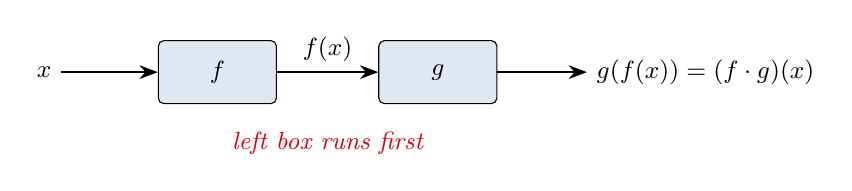
\begin{tikzpicture}[font=\small,>=Stealth,
  box/.style={draw,rounded corners=2pt,minimum width=1.5cm,minimum height=8mm,fill=armBlue!12}]
\node (x) at (0,0) {$x$};
\node[box] (f) at (2.2,0) {$f$};
\node[box] (g) at (5.0,0) {$g$};
\node (out) at (8.4,0) {$g(f(x))=(f\cdot g)(x)$};
\draw[->,thick] (x) -- (f);
\draw[->,thick] (f) -- node[above]{$f(x)$} (g);
\draw[->,thick] (g) -- (out);
\node[armRed] at (3.6,-0.9) {\itshape left box runs first};
\end{tikzpicture}
\end{center}

% ============================================================================
\section*{Problem 2 - Domain and range from a formula}

\begin{problembox}[2]
Let $f\subseteq\R\times\R$. Find the domain and the range for each formula:
\[
\text{(a) } x^2+3,\quad
\text{(b) } \sqrt{x-2},\quad
\text{(c) } \tfrac{1}{\sqrt{x-2}},\quad
\text{(d) } |x|,\quad
\text{(e) } \tfrac{1}{x^2+2},\quad
\text{(f) } \tfrac{1}{x^2-2}.
\]
\end{problembox}

\begin{ideabox}
Two separate questions, read off the graph. The \textbf{domain} is \textquotedbl{}where is the
formula legal\textquotedbl{}: avoid only two dangers, a \emph{negative under a square root} and a
\emph{zero in a denominator}; everything else is allowed, so the domain is all of $\R$ minus those
forbidden points. The \textbf{range} is \textquotedbl{}what heights does the graph reach\textquotedbl{}:
build it up from the inside out. For a formula like $\tfrac{1}{x^2-2}$, first see what
$u=x^2-2$ can be, then see what $\tfrac1u$ does to that set. The reciprocal flips the order of an
interval and sends values near $0$ to $\pm\infty$, which is exactly why the range of (f) splits
into two pieces.
\end{ideabox}

\textbf{Step 1 - Domains (find the forbidden points).}
(a),(d),(e) have no roots and no denominators, and $x^2+2\ge2>0$, so they are legal everywhere:
domain $\R$. For (b) $\sqrt{x-2}$ needs $x-2\ge0$, i.e. $x\ge2$. For (c) $\tfrac1{\sqrt{x-2}}$ needs
the root legal \emph{and} nonzero, so $x-2>0$, i.e. $x>2$. For (f) $\tfrac1{x^2-2}$ needs
$x^2-2\ne0$, i.e. $x\ne\pm\sqrt2$.

\textbf{Step 2 - Ranges (work inside out).}
(a) $x^2\ge0\Rightarrow x^2+3\ge3$, every value $\ge3$ is hit, range $[3,\infty)$.
(b) $\sqrt{\,\cdot\,}\ge0$ and grows without bound, range $[0,\infty)$.
(c) $\tfrac1{\sqrt{x-2}}>0$; as $x\to2^+$ it blows up, as $x\to\infty$ it tends to $0$ (never
reaching it), range $(0,\infty)$.
(d) $|x|\ge0$, range $[0,\infty)$.
(e) $x^2+2\in[2,\infty)$, so $\tfrac1{x^2+2}\in(0,\tfrac12]$; the maximum $\tfrac12$ is at $x=0$,
and the values shrink toward $0$ as $|x|\to\infty$. Range $\bigl(0,\tfrac12\bigr]$.
(f) Let $u=x^2-2$, so $u\in[-2,\infty)\setminus\{0\}$. On $u\in[-2,0)$ the reciprocal gives
$\tfrac1u\in(-\infty,-\tfrac12]$ (the value $-\tfrac12$ comes from $u=-2$, i.e. $x=0$); on
$u\in(0,\infty)$ it gives $\tfrac1u\in(0,\infty)$. Range
$\bigl(-\infty,-\tfrac12\bigr]\cup(0,\infty)$.

\textbf{Step 3 - Always check the boundary values.}
(e) at $x=0$: $\tfrac1{0+2}=\tfrac12$. \checkmark\ (f) at $x=0$: $\tfrac1{0-2}=-\tfrac12$, the top
of the negative branch. \checkmark\ Numeric sampling on a fine grid confirms every min/max above.

\answer{%
(a) $\dom=\R$, range $[3,\infty)$;\quad
(b) $\dom=[2,\infty)$, range $[0,\infty)$;\quad
(c) $\dom=(2,\infty)$, range $(0,\infty)$;\\[2pt]
(d) $\dom=\R$, range $[0,\infty)$;\quad
(e) $\dom=\R$, range $\bigl(0,\tfrac12\bigr]$;\quad
(f) $\dom=\R\setminus\{\pm\sqrt2\}$, range $\bigl(-\infty,-\tfrac12\bigr]\cup(0,\infty)$.}

\medskip
\textbf{Reading domain and range off the picture.} The two clearest cases, (b) and (f). For (b),
the domain is the bracket on the $x$-axis ($x\ge2$) and the range is the bracket on the $y$-axis
($y\ge0$). For (f), the curve has vertical asymptotes at $x=\pm\sqrt2$ and splits the $y$-axis into
exactly the two range pieces.

\begin{center}
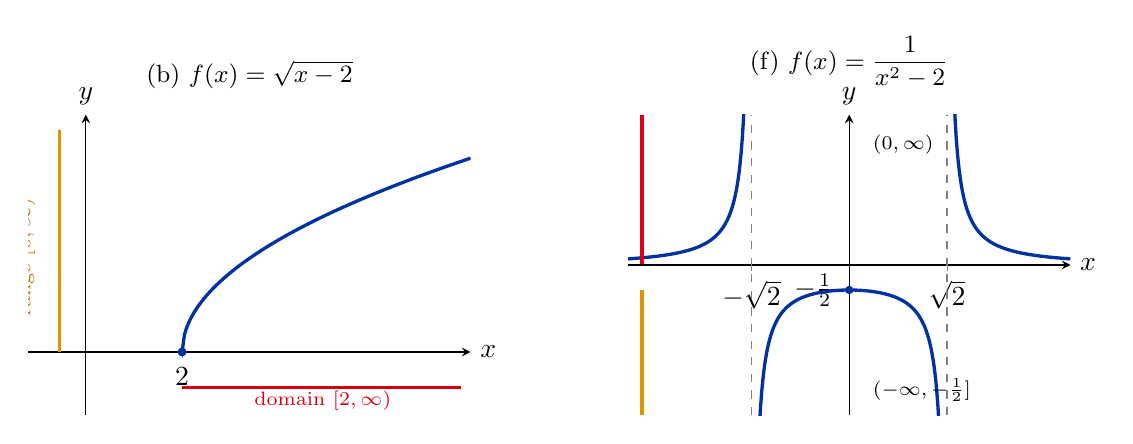
\begin{tikzpicture}
\begin{axis}[
  name=plotb, width=7.2cm, height=5.4cm,
  axis lines=middle, xlabel={$x$}, ylabel={$y$},
  xmin=-1.2, xmax=8, ymin=-0.8, ymax=3,
  xtick={2}, ytick={0}, xticklabels={$2$},
  title={(b) $f(x)=\sqrt{x-2}$}, title style={font=\small},
  every axis x label/.style={at={(ticklabel* cs:1.0)},anchor=west},
  every axis y label/.style={at={(ticklabel* cs:1.0)},anchor=south}]
\addplot[domain=2:8, samples=120, very thick, armBlue]{sqrt(x-2)};
\addplot[only marks, mark=*, mark size=1.4pt, armBlue] coordinates {(2,0)};
% domain bracket on x-axis
\draw[armRed, very thick] (axis cs:2,-0.45) -- (axis cs:7.8,-0.45);
\node[armRed,font=\scriptsize,anchor=west] at (axis cs:3.3,-0.62) {domain $[2,\infty)$};
% range bracket on y-axis
\draw[armOrange!90!black, very thick] (axis cs:-0.55,0) -- (axis cs:-0.55,2.8);
\node[armOrange!75!black,font=\scriptsize,rotate=90,anchor=south] at (axis cs:-0.85,1.2) {range $[0,\infty)$};
\end{axis}

\begin{axis}[
  name=plotf, at={($(plotb.east)+(2.0cm,0)$)}, anchor=west,
  width=7.2cm, height=5.4cm,
  axis lines=middle, xlabel={$x$}, ylabel={$y$},
  xmin=-3.2, xmax=3.2, ymin=-3, ymax=3,
  xtick={-1.414,1.414}, xticklabels={$-\sqrt2$,$\sqrt2$},
  ytick={-0.5}, yticklabels={$-\tfrac12$},
  title={(f) $f(x)=\dfrac{1}{x^2-2}$}, title style={font=\small},
  every axis x label/.style={at={(ticklabel* cs:1.0)},anchor=west},
  every axis y label/.style={at={(ticklabel* cs:1.0)},anchor=south}]
% positive branches (|x|>sqrt2)
\addplot[domain=1.46:3.2, samples=120, very thick, armBlue]{1/(x^2-2)};
\addplot[domain=-3.2:-1.46, samples=120, very thick, armBlue]{1/(x^2-2)};
% negative branch (|x|<sqrt2)
\addplot[domain=-1.37:1.37, samples=160, very thick, armBlue]{1/(x^2-2)};
\addplot[only marks, mark=*, mark size=1.3pt, armBlue] coordinates {(0,-0.5)};
\draw[dashed, gray] (axis cs:-1.414,-3) -- (axis cs:-1.414,3);
\draw[dashed, gray] (axis cs: 1.414,-3) -- (axis cs: 1.414,3);
% range pieces on y-axis
\draw[armOrange!90!black, very thick] (axis cs:-3.0,-3) -- (axis cs:-3.0,-0.5);
\draw[armRed, very thick] (axis cs:-3.0,0.02) -- (axis cs:-3.0,3);
\node[font=\scriptsize,anchor=west] at (axis cs:0.2,2.4) {$(0,\infty)$};
\node[font=\scriptsize,anchor=west] at (axis cs:0.2,-2.5) {$(-\infty,-\tfrac12]$};
\end{axis}
\end{tikzpicture}
\end{center}

\begin{methodbox}
\textbf{Transferable technique:} domain $=$ \textquotedbl{}all $x$ except where a root goes
negative or a denominator is zero.\textquotedbl{} Range $=$ build the value set \emph{inside out}:
track what the inner expression ($x^2$, $x-2$, $x^2-2$) can be, then apply the outer operation
($+3$, $\sqrt{\;}$, reciprocal). The reciprocal is the tricky one: it sends $(0,M]$ to
$[\tfrac1M,\infty)$ and a set straddling $0$ to two separate pieces.
\end{methodbox}

% ============================================================================
\section*{Problem 4 - Compositions $f\cdot g$ and $g\cdot f$}

\begin{problembox}[4]
Let $f,g:\R\to\R$. Find $f\cdot g$ and $g\cdot f$ (course convention $(f\cdot g)(x)=g(f(x))$,
apply $f$ first):
\[
\text{(a) } f(x)=x^2+1,\ g(x)=x+3;\qquad
\text{(b) } f(x)=\sqrt{x^2+2},\ g(x)=x^2+3;
\]
\[
\text{(c) } f(x)=\tfrac1x,\ g(x)=2x+3.
\]
\end{problembox}

\begin{ideabox}
Composition is just plugging one machine's output into the next machine. The only thing to get
right is \emph{which machine runs first}. Under the course's left-to-right rule, $f\cdot g$ runs
$f$ first: take $x$, compute $f(x)$, then feed that into $g$, giving $g(f(x))$. So to build
$f\cdot g$, write down $g(\square)$ and replace every $\square$ by the whole formula for $f(x)$.
Order matters: in general $f\cdot g\ne g\cdot f$, and part (a) shows that loudly.
\end{ideabox}

\textbf{Step 1 - Fix the recipe.} $(f\cdot g)(x)=g(f(x))$ (substitute $f$ into $g$);
$(g\cdot f)(x)=f(g(x))$ (substitute $g$ into $f$).

\textbf{Step 2 - Part (a).} $f(x)=x^2+1$, $g(x)=x+3$.
\[
(f\cdot g)(x)=g(f(x))=\underbrace{(x^2+1)}_{f(x)}+3=x^2+4,\qquad
(g\cdot f)(x)=f(g(x))=\underbrace{(x+3)}_{g(x)}{}^2+1=x^2+6x+10.
\]
The two are different ($x^2+4\ne x^2+6x+10$), the headline lesson of this problem.

\textbf{Step 3 - Part (b).} $f(x)=\sqrt{x^2+2}$, $g(x)=x^2+3$.
\[
(f\cdot g)(x)=g(f(x))=\bigl(\sqrt{x^2+2}\bigr)^2+3=(x^2+2)+3=x^2+5,
\]
\[
(g\cdot f)(x)=f(g(x))=\sqrt{(x^2+3)^2+2}.
\]
The square and the square root cancel cleanly in $f\cdot g$ because $x^2+2\ge0$.

\textbf{Step 4 - Part (c).} $f(x)=\tfrac1x$, $g(x)=2x+3$.
\[
(f\cdot g)(x)=g(f(x))=2\cdot\tfrac1x+3=\tfrac2x+3,\qquad
(g\cdot f)(x)=f(g(x))=\tfrac{1}{2x+3}.
\]

\textbf{Step 5 - Always check at a sample point.} (a) at $x=1$: $f(1)=2$, $g(2)=5$, and
$1^2+4=5$. \checkmark\ For $g\cdot f$: $g(1)=4$, $f(4)=17$, and $1+6+10=17$. \checkmark\ All three
parts and both orders were confirmed numerically at many points.

\answer{%
(a) $f\cdot g=x^2+4$,\ \ $g\cdot f=x^2+6x+10$;\quad
(b) $f\cdot g=x^2+5$,\ \ $g\cdot f=\sqrt{(x^2+3)^2+2}$;\quad
(c) $f\cdot g=\tfrac2x+3$,\ \ $g\cdot f=\tfrac1{2x+3}$.}

\medskip
\textbf{The arrow chain that makes the order unmistakable.} For (a) at the sample $x=1$, the two
compositions trace different paths. Top row is $f\cdot g$ (the course order, $f$ first); bottom row
is $g\cdot f$.

\begin{center}
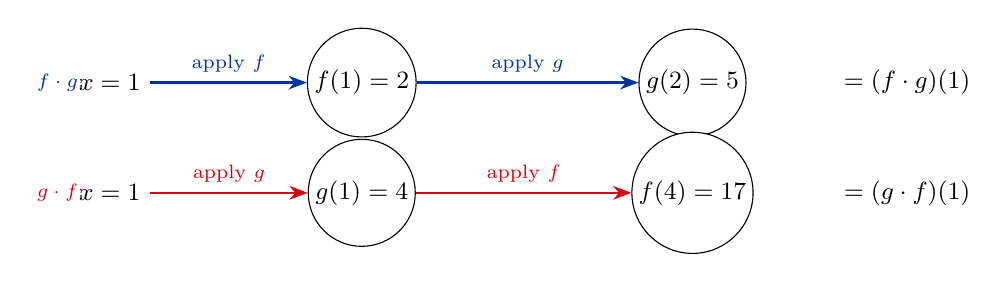
\begin{tikzpicture}[font=\small,>=Stealth, node distance=14mm,
  val/.style={draw,circle,inner sep=1.6pt,fill=white},
  op/.style={midway,above,font=\scriptsize}]
% f.g : x -> f -> g
\node (a0) at (0,1.4) {$x=1$};
\node[val] (a1) at (3.2,1.4) {$f(1)=2$};
\node[val] (a2) at (7.4,1.4) {$g(2)=5$};
\node[anchor=west] at (9.2,1.4) {$=(f\cdot g)(1)$};
\draw[->,thick,armBlue] (a0) -- node[op]{apply $f$} (a1);
\draw[->,thick,armBlue] (a1) -- node[op]{apply $g$} (a2);
\node[armBlue,font=\scriptsize,anchor=east] at (-0.2,1.4) {$f\cdot g$:};
% g.f : x -> g -> f
\node (b0) at (0,0) {$x=1$};
\node[val] (b1) at (3.2,0) {$g(1)=4$};
\node[val] (b2) at (7.4,0) {$f(4)=17$};
\node[anchor=west] at (9.2,0) {$=(g\cdot f)(1)$};
\draw[->,thick,armRed] (b0) -- node[op]{apply $g$} (b1);
\draw[->,thick,armRed] (b1) -- node[op]{apply $f$} (b2);
\node[armRed,font=\scriptsize,anchor=east] at (-0.2,0) {$g\cdot f$:};
\end{tikzpicture}
\end{center}
Same start $x=1$, different finishes ($5$ vs $17$): composition is not commutative, and the
left-to-right rule tells you which box fires first.

\begin{methodbox}
\textbf{Transferable technique:} to build $f\cdot g$ (course order), write the \emph{second}
function $g(\square)$ and substitute the \emph{whole} first formula for $\square$. Always sanity
check at one number by literally walking the pipeline. If your two compositions come out equal for
a generic pair of functions, you almost certainly mixed up the order.
\end{methodbox}

% ============================================================================
\section*{Problem 5 - Inverse functions}

\begin{problembox}[5]
Find the inverse function for each:
\[
\text{(a) } f(x)=\frac{x+4}{2},\qquad
\text{(b) } f(x)=x^3,\qquad
\text{(c) } f(x)=\frac{x-2}{x+3}.
\]
\end{problembox}

\begin{ideabox}
The inverse $f^{-1}$ undoes $f$: if $f$ sends $x$ to $y$, then $f^{-1}$ sends $y$ back to $x$. To
find a formula, just \emph{solve $y=f(x)$ for $x$}. Whatever you get, $x=(\text{expression in }y)$,
is $f^{-1}(y)$; rename $y$ to $x$ at the end if you like. Geometrically the inverse is the
\textbf{mirror image of the graph across the line $y=x$}, because swapping the roles of input and
output swaps the two axes.
\end{ideabox}

\textbf{Step 1 - Part (a).} Solve $y=\tfrac{x+4}{2}$: multiply by $2$, $2y=x+4$, so $x=2y-4$.
Hence $f^{-1}(x)=2x-4$.

\textbf{Step 2 - Part (b).} Solve $y=x^3$: take the (real) cube root, $x=\sqrt[3]{y}$. Hence
$f^{-1}(x)=\sqrt[3]{x}$. (Cube root is defined for all reals, including negatives, so this is a
genuine inverse on all of $\R$ - which works precisely because $x^3:\R\to\R$ is a bijection, as
Problem 6(c) confirms.)

\textbf{Step 3 - Part (c).} Solve $y=\tfrac{x-2}{x+3}$. Clear the denominator:
$y(x+3)=x-2\Rightarrow yx+3y=x-2\Rightarrow x(y-1)=-2-3y$, so
\[
x=\frac{-2-3y}{y-1}=\frac{3y+2}{1-y}.
\]
Hence $f^{-1}(x)=\dfrac{3x+2}{1-x}$ (defined for $x\ne1$; the value $1$ is exactly the height the
graph never reaches, its horizontal asymptote).

\textbf{Step 4 - Always check: $f^{-1}$ really undoes $f$.}
(a) $f^{-1}(f(x))=2\cdot\tfrac{x+4}{2}-4=(x+4)-4=x$. \checkmark\
(c) take $x=0$: $f(0)=\tfrac{-2}{3}$, then $f^{-1}\!\bigl(-\tfrac23\bigr)
=\tfrac{3(-2/3)+2}{1-(-2/3)}=\tfrac{0}{5/3}=0$. \checkmark\ Both directions verified numerically.

\answer{(a) $f^{-1}(x)=2x-4$;\quad (b) $f^{-1}(x)=\sqrt[3]{x}$;\quad
(c) $f^{-1}(x)=\dfrac{3x+2}{1-x}$ \ (for $x\ne1$).}

\medskip
\textbf{The inverse is a reflection across $y=x$.} Here is part (a): the line $f(x)=\tfrac{x+4}{2}$
and its inverse $f^{-1}(x)=2x-4$ are mirror images in the dashed diagonal. Pick any point on one
graph, swap its coordinates, and you land on the other.

\begin{center}
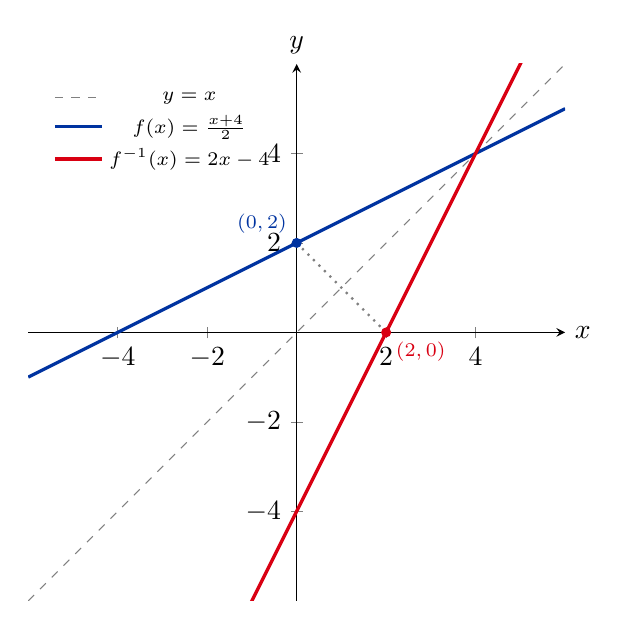
\begin{tikzpicture}
\begin{axis}[
  width=8.4cm, height=8.4cm, axis equal image,
  axis lines=middle, xlabel={$x$}, ylabel={$y$},
  xmin=-6, xmax=6, ymin=-6, ymax=6,
  xtick={-4,-2,2,4}, ytick={-4,-2,2,4},
  legend pos=north west, legend style={font=\scriptsize, draw=none, fill=none},
  every axis x label/.style={at={(ticklabel* cs:1.0)},anchor=west},
  every axis y label/.style={at={(ticklabel* cs:1.0)},anchor=south}]
\addplot[domain=-6:6, samples=2, dashed, gray]{x};
\addlegendentry{$y=x$}
\addplot[domain=-6:6, samples=2, very thick, armBlue]{(x+4)/2};
\addlegendentry{$f(x)=\tfrac{x+4}{2}$}
\addplot[domain=-6:6, samples=2, very thick, armRed]{2*x-4};
\addlegendentry{$f^{-1}(x)=2x-4$}
% a matched pair of mirror points: (0,2) on f, (2,0) on f^{-1}
\addplot[only marks, mark=*, mark size=1.6pt, armBlue] coordinates {(0,2)};
\addplot[only marks, mark=*, mark size=1.6pt, armRed] coordinates {(2,0)};
\draw[dotted, thick, gray] (axis cs:0,2) -- (axis cs:2,0);
\node[font=\scriptsize, armBlue, anchor=south east] at (axis cs:0,2) {$(0,2)$};
\node[font=\scriptsize, armRed, anchor=north west] at (axis cs:2,0) {$(2,0)$};
\end{axis}
\end{tikzpicture}
\end{center}

\begin{methodbox}
\textbf{Transferable technique:} to invert, \emph{solve $y=f(x)$ for $x$}. For a fraction
$\tfrac{ax+b}{cx+d}$, cross-multiply and collect all $x$ terms on one side. Check by composing:
$f^{-1}(f(x))$ must simplify to $x$. The inverse graph is always the reflection of $f$ across
$y=x$.
\end{methodbox}

% ============================================================================
\section*{Problem 6 - Injective, surjective, bijective ($f:\R\to\R$)}

\begin{problembox}[6]
Decide which of the maps $f:\R\to\R$ are injective, surjective, or bijective:
\[
\text{(a) } |x|,\quad
\text{(b) } x^2+4,\quad
\text{(c) } x^3+6,\quad
\text{(d) } x+|x|,\quad
\text{(e) } x(x-2)(x+2).
\]
\end{problembox}

\begin{ideabox}
Two independent questions, and each has a one-line picture test.
\textbf{Injective} (\textquotedbl{}one-to-one\textquotedbl{}) means \emph{different inputs give
different outputs}: no two $x$ values share a height. Picture test: every \textbf{horizontal line}
hits the graph \emph{at most once}. If even one horizontal line cuts the graph twice, injectivity
fails. \textbf{Surjective} (\textquotedbl{}onto $\R$\textquotedbl{}) means \emph{every} target
height is reached: the range is all of $\R$. Picture test: every horizontal line hits the graph
\emph{at least once}. \textbf{Bijective} $=$ both $=$ every horizontal line hits \emph{exactly
once} (and then $f$ has an inverse). The classic killers: a $|x|$ or even power folds the line in
half (kills injectivity and surjectivity); an odd power like $x^3$ is a clean increasing curve
(bijective).
\end{ideabox}

\textbf{Step 1 - The horizontal-line test, function by function.}
\begin{itemize}[leftmargin=1.4em,itemsep=1pt]
\item[(a)] $|x|$: the line $y=1$ meets it at $x=\pm1$ (two points) $\Rightarrow$ \emph{not}
injective; the line $y=-1$ meets it nowhere ($|x|\ge0$) $\Rightarrow$ \emph{not} surjective.
\textbf{Neither.}
\item[(b)] $x^2+4$: $f(1)=f(-1)=5$ $\Rightarrow$ not injective; range is $[4,\infty)$, so $y=0$ is
never reached $\Rightarrow$ not surjective. \textbf{Neither.}
\item[(c)] $x^3+6$: strictly increasing (if $x_1<x_2$ then $x_1^3<x_2^3$), so every horizontal
line meets it at most once $\Rightarrow$ injective; as $x\to\pm\infty$ the value runs over all of
$\R$, so every line meets it at least once $\Rightarrow$ surjective. \textbf{Bijective}, with
inverse $f^{-1}(x)=\sqrt[3]{x-6}$.
\item[(d)] $x+|x|$: for $x\le0$ this is $x+(-x)=0$, so the whole ray $x\le0$ maps to $0$
$\Rightarrow$ badly non-injective; the output is never negative (it equals $0$ or $2x>0$)
$\Rightarrow$ range $[0,\infty)$, not surjective. \textbf{Neither.}
\item[(e)] $x(x-2)(x+2)=x^3-4x$: it is a cubic, so as $x\to\pm\infty$ it covers all of $\R$
$\Rightarrow$ surjective; but $f(0)=f(2)=f(-2)=0$, so the line $y=0$ meets it three times
$\Rightarrow$ not injective. \textbf{Surjective only.}
\end{itemize}

\textbf{Step 2 - Always check the witnesses.} The non-injective verdicts each rest on a concrete
collision: $|{-1}|=|1|$, $(-1)^2+4=1^2+4$, $f(-2)=f(0)$ in (d), and $(-2)(-4)(0)=0=2\cdot0\cdot4$
in (e). The non-surjective verdicts rest on a missed target ($y=-1$ for (a), $y=0$ for (b)/(d)).
For (c) the cube-root formula explicitly produces a preimage for every target. All confirmed by
dense sampling.

\answer{%
(a) neither;\quad (b) neither;\quad \textbf{(c) bijective};\quad
(d) neither;\quad (e) surjective but not injective.}

\medskip
\textbf{The showpiece: arrow diagrams and the horizontal-line test.} First, the three pictures
every student should carry in their head. Dots on the left are inputs, dots on the right are
targets; an arrow is $x\mapsto f(x)$.

\begin{center}
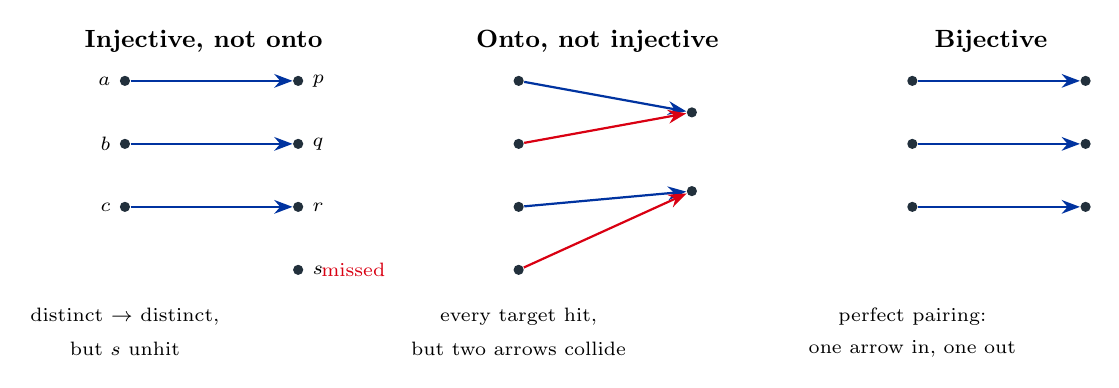
\begin{tikzpicture}[font=\scriptsize,>=Stealth,
  dot/.style={circle,fill=ink,inner sep=1.3pt},
  every node/.style={inner sep=1pt}]
\def\dx{2.2}
% --- INJECTIVE not surjective ---
\begin{scope}[shift={(0,0)}]
  \node[font=\small\bfseries] at (1.0,2.5) {Injective, not onto};
  \foreach \y/\n in {2/a,1.2/b,0.4/c} {\node[dot] (L\n) at (0,\y) {}; \node[left=2pt of L\n]{$\n$};}
  \foreach \y/\n in {2/p,1.2/q,0.4/r,-0.4/s} {\node[dot] (R\n) at (\dx,\y) {}; \node[right=2pt of R\n,font=\scriptsize]{$\n$};}
  \draw[->,armBlue,thick] (La) -- (Rp);
  \draw[->,armBlue,thick] (Lb) -- (Rq);
  \draw[->,armBlue,thick] (Lc) -- (Rr);
  \node[armRed] at (\dx+0.7,-0.4) {missed};
  \node at (0,-1.0) {distinct $\to$ distinct,};
  \node at (0,-1.4) {but $s$ unhit};
\end{scope}
% --- SURJECTIVE not injective ---
\begin{scope}[shift={(5.0,0)}]
  \node[font=\small\bfseries] at (1.0,2.5) {Onto, not injective};
  \foreach \y/\n in {2/a,1.2/b,0.4/c,-0.4/d} {\node[dot] (L\n) at (0,\y) {};}
  \foreach \y/\n in {1.6/p,0.6/q} {\node[dot] (R\n) at (\dx,\y) {};}
  \draw[->,armBlue,thick] (La) -- (Rp);
  \draw[->,armRed,thick]  (Lb) -- (Rp);
  \draw[->,armBlue,thick] (Lc) -- (Rq);
  \draw[->,armRed,thick]  (Ld) -- (Rq);
  \node at (0,-1.0) {every target hit,};
  \node at (0,-1.4) {but two arrows collide};
\end{scope}
% --- BIJECTIVE ---
\begin{scope}[shift={(10.0,0)}]
  \node[font=\small\bfseries] at (1.0,2.5) {Bijective};
  \foreach \y/\n in {2/a,1.2/b,0.4/c} {\node[dot] (L\n) at (0,\y) {};}
  \foreach \y/\n in {2/p,1.2/q,0.4/r} {\node[dot] (R\n) at (\dx,\y) {};}
  \draw[->,armBlue,thick] (La) -- (Rp);
  \draw[->,armBlue,thick] (Lb) -- (Rq);
  \draw[->,armBlue,thick] (Lc) -- (Rr);
  \node at (0,-1.0) {perfect pairing:};
  \node at (0,-1.4) {one arrow in, one out};
\end{scope}
\end{tikzpicture}
\end{center}

Now the horizontal-line test applied to the two contrasting graphs from this problem: $x^2+4$
(folded, a line can cut twice) versus $x^3+6$ (monotone, every line cuts exactly once).

\begin{center}
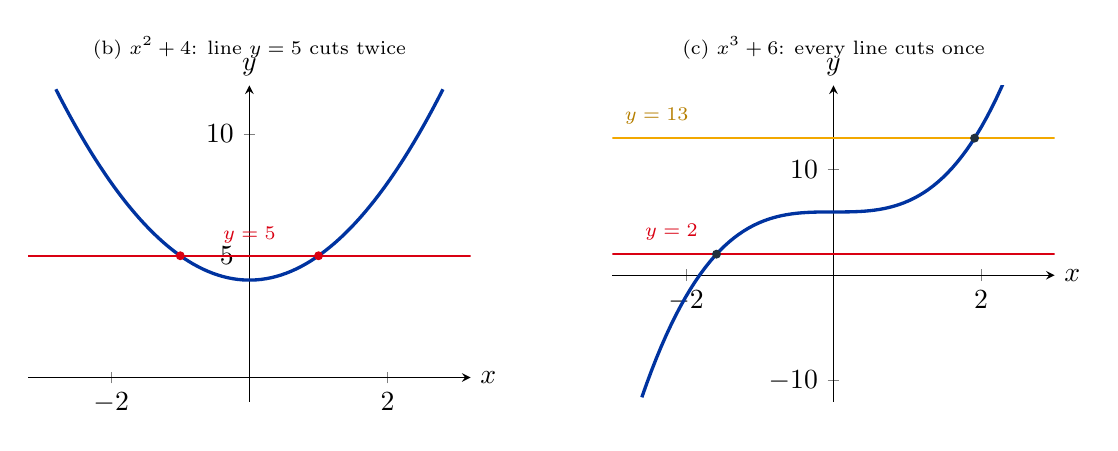
\begin{tikzpicture}
\begin{axis}[
  name=p1, width=7.2cm, height=5.6cm, axis lines=middle,
  xlabel={$x$}, ylabel={$y$}, xmin=-3.2, xmax=3.2, ymin=-1, ymax=12,
  title={(b) $x^2+4$: line $y=5$ cuts twice}, title style={font=\scriptsize},
  every axis x label/.style={at={(ticklabel* cs:1.0)},anchor=west},
  every axis y label/.style={at={(ticklabel* cs:1.0)},anchor=south}]
\addplot[domain=-2.8:2.8, samples=80, very thick, armBlue]{x^2+4};
\addplot[domain=-3.2:3.2, samples=2, armRed, thick]{5};
\addplot[only marks, mark=*, mark size=1.4pt, armRed] coordinates {(-1,5)(1,5)};
\node[font=\scriptsize, armRed, anchor=south] at (axis cs:0,5.1) {$y=5$};
\end{axis}
\begin{axis}[
  name=p2, at={($(p1.east)+(1.8cm,0)$)}, anchor=west,
  width=7.2cm, height=5.6cm, axis lines=middle,
  xlabel={$x$}, ylabel={$y$}, xmin=-3, xmax=3, ymin=-12, ymax=18,
  title={(c) $x^3+6$: every line cuts once}, title style={font=\scriptsize},
  every axis x label/.style={at={(ticklabel* cs:1.0)},anchor=west},
  every axis y label/.style={at={(ticklabel* cs:1.0)},anchor=south}]
\addplot[domain=-2.6:2.6, samples=80, very thick, armBlue]{x^3+6};
\addplot[domain=-3:3, samples=2, armRed, thick]{2};
\addplot[domain=-3:3, samples=2, armOrange, thick]{13};
\addplot[only marks, mark=*, mark size=1.4pt, ink] coordinates {(-1.587,2)(1.913,13)};
\node[font=\scriptsize, armRed, anchor=south] at (axis cs:-2.2,2.4) {$y=2$};
\node[font=\scriptsize, armOrange!75!black, anchor=south] at (axis cs:-2.4,13.4) {$y=13$};
\end{axis}
\end{tikzpicture}
\end{center}

\begin{methodbox}
\textbf{Transferable technique:} to disprove injectivity, exhibit one collision $f(a)=f(b)$ with
$a\ne b$. To disprove surjectivity, exhibit one unreached target. To prove bijectivity of a real
function, show it is strictly monotone (injective) and runs from $-\infty$ to $+\infty$
(surjective) - then it has an inverse. Even powers and $|x|$ fold; odd powers do not.
\end{methodbox}

% ============================================================================
\section*{Problem 10 - $\Ker(f)$ is an equivalence relation}

\begin{problembox}[10]
Show that for any function $f:A\to B$, its \textbf{kernel}
$\Ker(f)=\{(x,y)\in A\times A: f(x)=f(y)\}$ is an equivalence relation on $A$.
\end{problembox}

\begin{ideabox}
The kernel relates two inputs exactly when they have the \emph{same output}. But \textquotedbl{}having
the same value\textquotedbl{} is built straight out of \emph{equality} ($=$) of those values, and
equality is the most equivalence-like relation there is: anything equals itself, equality is
symmetric, and it chains. So $\Ker(f)$ inherits all three properties of $=$ for free. The payoff
picture: $\Ker(f)$ chops the domain into \textbf{fibers}, one clump per output value, where a fiber
$f^{-1}(b)$ is all inputs that $f$ sends to $b$. Equivalence classes $=$ fibers.
\end{ideabox}

\textbf{Step 1 - Reflexive.} For any $x\in A$, $f(x)=f(x)$ trivially, so $(x,x)\in\Ker(f)$.

\textbf{Step 2 - Symmetric.} If $(x,y)\in\Ker(f)$ then $f(x)=f(y)$; equality is symmetric, so
$f(y)=f(x)$, hence $(y,x)\in\Ker(f)$.

\textbf{Step 3 - Transitive.} If $(x,y),(y,z)\in\Ker(f)$ then $f(x)=f(y)$ and $f(y)=f(z)$; chaining
equalities gives $f(x)=f(z)$, hence $(x,z)\in\Ker(f)$.

\textbf{Step 4 - Conclusion and the fiber picture.} All three hold, so $\Ker(f)$ is an equivalence
relation. Its equivalence class of $x$ is $\{y:f(y)=f(x)\}=f^{-1}(f(x))$, the fiber over the value
$f(x)$. These fibers partition $A$: every input lands in exactly one fiber (its own output), and
different output values give disjoint fibers.

\answer{$\Ker(f)$ is reflexive, symmetric, and transitive (inherited from $=$ on $B$), hence an
equivalence relation on $A$; its classes are the fibers $f^{-1}(b)$.}

\medskip
\textbf{The fiber partition.} Take the toy map $f:\{1,2,3,4,5,6\}\to\{p,q,r\}$ with
$f(1)=f(2)=f(3)=p$, $f(4)=f(5)=q$, $f(6)=r$. The kernel partitions the domain into three fibers,
one per value. Two inputs are $\Ker(f)$-related iff they sit in the same shaded clump.

\begin{center}
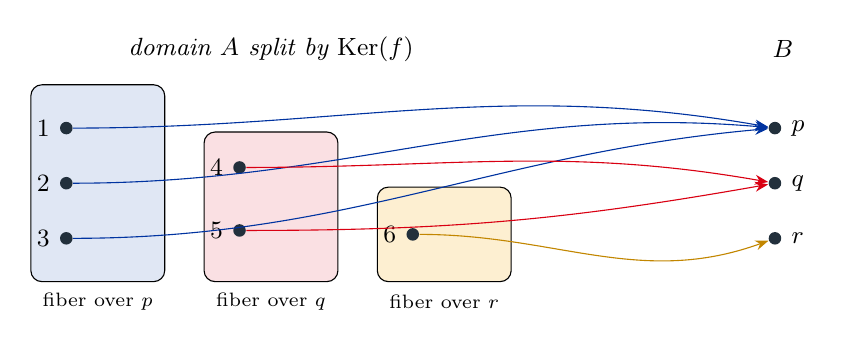
\begin{tikzpicture}[font=\small,>=Stealth,
  dot/.style={circle,fill=ink,inner sep=1.6pt}]
% domain A with three fibers
\begin{scope}
  \node[draw,rounded corners,fill=armBlue!12,minimum width=1.7cm,minimum height=2.5cm] (f1) at (0,0) {};
  \node[draw,rounded corners,fill=armRed!12,minimum width=1.7cm,minimum height=1.9cm] (f2) at (2.2,-0.3) {};
  \node[draw,rounded corners,fill=armOrange!18,minimum width=1.7cm,minimum height=1.2cm] (f3) at (4.4,-0.65) {};
  \node[dot,label=left:$1$] (n1) at (-0.4,0.7) {};
  \node[dot,label=left:$2$] (n2) at (-0.4,0.0) {};
  \node[dot,label=left:$3$] (n3) at (-0.4,-0.7) {};
  \node[dot,label=left:$4$] (n4) at (1.8,0.2) {};
  \node[dot,label=left:$5$] (n5) at (1.8,-0.6) {};
  \node[dot,label=left:$6$] (n6) at (4.0,-0.65) {};
  \node[font=\scriptsize] at (0,-1.5) {fiber over $p$};
  \node[font=\scriptsize] at (2.2,-1.5) {fiber over $q$};
  \node[font=\scriptsize] at (4.4,-1.5) {fiber over $r$};
  \node[font=\small\itshape] at (2.2,1.7) {domain $A$ split by $\Ker(f)$};
\end{scope}
% codomain B
\begin{scope}[shift={(8.6,0)}]
  \node[dot,label=right:$p$] (bp) at (0,0.7) {};
  \node[dot,label=right:$q$] (bq) at (0,0.0) {};
  \node[dot,label=right:$r$] (br) at (0,-0.7) {};
  \node[font=\small\itshape] at (0.1,1.7) {$B$};
\end{scope}
% arrows
\draw[->,armBlue]   (n1) to[out=0,in=170] (bp);
\draw[->,armBlue]   (n2) to[out=0,in=175] (bp);
\draw[->,armBlue]   (n3) to[out=0,in=185] (bp);
\draw[->,armRed]    (n4) to[out=0,in=170] (bq);
\draw[->,armRed]    (n5) to[out=0,in=190] (bq);
\draw[->,armOrange!80!black] (n6) to[out=0,in=200] (br);
\end{tikzpicture}
\end{center}

\begin{methodbox}
\textbf{Transferable technique:} any relation of the form \textquotedbl{}$x\sim y$ iff
$g(x)=g(y)$\textquotedbl{} (\textquotedbl{}same value of some quantity\textquotedbl{}) is
automatically an equivalence relation, because it is pulled back from $=$. Its classes are the
level sets / fibers of $g$. This is the single most common way equivalence relations arise.
\end{methodbox}

% ============================================================================
\section*{Problem 12 - $f(x)=\dfrac{x}{2x+1}$ on $\Q^+$ is injective but not surjective}

\begin{problembox}[12]
Let $f:\Q^+\to\Q^+$ be $f(x)=\dfrac{x}{2x+1}$. Show that $f$ is injective but not surjective.
\end{problembox}

\begin{ideabox}
\textbf{Injective} is pure algebra: assume two inputs give the same output and grind the equation
until it forces the inputs equal. \textbf{Not surjective} needs a target with no preimage, and the
clean way to find one is to \emph{bound the range}. For positive $x$, the denominator $2x+1$ is a
bit bigger than $2x$, so $\tfrac{x}{2x+1}$ is a bit smaller than $\tfrac{x}{2x}=\tfrac12$. Every
output is therefore strictly below $\tfrac12$. So anything $\ge\tfrac12$ (e.g. the value $1$, which
is in $\Q^+$) is unreachable - surjectivity fails by a wide margin.
\end{ideabox}

\textbf{Step 1 - Injective.} Suppose $f(x)=f(y)$, i.e. $\dfrac{x}{2x+1}=\dfrac{y}{2y+1}$.
Cross-multiply (both denominators are positive): $x(2y+1)=y(2x+1)$, so $2xy+x=2xy+y$, hence
$x=y$. Distinct inputs cannot share an output, so $f$ is injective.

\textbf{Step 2 - Bound the range.} For $x\in\Q^+$ we have $x>0$, so $2x+1>2x>0$ and therefore
\[
f(x)=\frac{x}{2x+1}<\frac{x}{2x}=\frac12.
\]
Also $f(x)>0$. So the entire range sits inside the open interval $\bigl(0,\tfrac12\bigr)$.

\textbf{Step 3 - Exhibit a missed target.} The number $1\in\Q^+$ satisfies $1\ge\tfrac12$, so it is
outside $(0,\tfrac12)$ and cannot be a value of $f$. (Algebraically: $\tfrac{x}{2x+1}=1$ forces
$x=2x+1$, i.e. $x=-1\notin\Q^+$.) Hence $f$ is \emph{not} surjective.

\textbf{Step 4 - Always check the bound is tight but never attained.} As $x\to\infty$,
$f(x)=\tfrac{x}{2x+1}\to\tfrac12$ from below (e.g. $f(10000)\approx0.49998$), so $\tfrac12$ is the
supremum but is never reached either - confirming the range is strictly inside $(0,\tfrac12)$.

\answer{Injective: $f(x)=f(y)\Rightarrow x=y$. Not surjective: every value is $<\tfrac12$, so e.g.
$1$ (and any value $\ge\tfrac12$) has no preimage.}

\medskip
\textbf{The range sits below $y=\tfrac12$.} Plotting $f$ for $x>0$, the curve climbs from $0$ but
stays under the dashed ceiling $y=\tfrac12$ forever. The whole target band $\bigl[\tfrac12,\infty\bigr)$
of $\Q^+$ - including $1$ - is empty of values.

\begin{center}
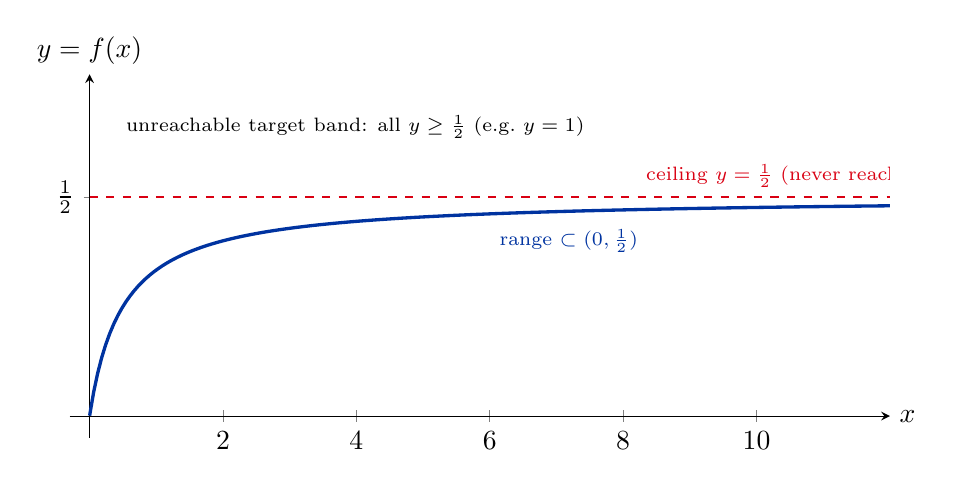
\begin{tikzpicture}
\begin{axis}[
  width=12cm, height=6.2cm, axis lines=middle,
  xlabel={$x$}, ylabel={$y=f(x)$}, xmin=-0.3, xmax=12, ymin=-0.05, ymax=0.78,
  ytick={0.5}, yticklabels={$\tfrac12$}, xtick={0,2,4,6,8,10},
  every axis x label/.style={at={(ticklabel* cs:1.0)},anchor=west},
  every axis y label/.style={at={(ticklabel* cs:1.0)},anchor=south}]
% horizontal asymptote / ceiling
\addplot[domain=0:12, samples=2, dashed, armRed, thick]{0.5};
\node[font=\scriptsize, armRed, anchor=south west] at (axis cs:8.2,0.5) {ceiling $y=\tfrac12$ (never reached)};
% the function
\addplot[domain=0.001:12, samples=200, very thick, armBlue]{x/(2*x+1)};
% the unreachable band sits at and above the ceiling y=1/2
\node[font=\scriptsize, anchor=west] at (axis cs:0.4,0.66) {unreachable target band: all $y\ge\tfrac12$ (e.g.\ $y=1$)};
\node[font=\scriptsize, armBlue, anchor=west] at (axis cs:6,0.40) {range $\subset(0,\tfrac12)$};
\end{axis}
\end{tikzpicture}
\end{center}

\begin{methodbox}
\textbf{Transferable technique:} to show \textquotedbl{}not surjective,\textquotedbl{} \emph{bound
the range} and name one target outside the bound. The estimate $\tfrac{x}{2x+1}<\tfrac{x}{2x}$
(shrink the denominator's $+1$) is the workhorse trick for rational functions. Injectivity for a
ratio is usually a one-line cross-multiplication.
\end{methodbox}

% ============================================================================
\section*{Problem 19 - When is $f(A\cap B)=f(A)\cap f(B)$?}

\begin{problembox}[19]
For which functions $f$ does $f(A\cap B)=f(A)\cap f(B)$ hold for all sets $A,B$?
\end{problembox}

\begin{ideabox}
One inclusion is free, the other costs injectivity. \emph{Free direction:} if $x\in A\cap B$ then
$f(x)$ is both in $f(A)$ and in $f(B)$, so $f(A\cap B)\subseteq f(A)\cap f(B)$ \emph{always}. The
reverse can fail because $f(A)\cap f(B)$ collects \textbf{shared output values}, which can come
from \emph{different} inputs - one input in $A$, a different one in $B$ - that need not meet in
$A\cap B$. Exactly when $f$ is \textbf{injective}, a shared output forces a shared input, and the
two sides become equal. So the identity holds for all $A,B$ \textbf{iff $f$ is injective}.
\end{ideabox}

\textbf{Step 1 - The always-true inclusion.} Let $y\in f(A\cap B)$, so $y=f(x)$ with
$x\in A\cap B$. Then $x\in A$ gives $y\in f(A)$, and $x\in B$ gives $y\in f(B)$, so
$y\in f(A)\cap f(B)$. Hence $f(A\cap B)\subseteq f(A)\cap f(B)$ for \emph{every} $f$.

\textbf{Step 2 - If $f$ is injective, the reverse holds.} Let $y\in f(A)\cap f(B)$, so
$y=f(a)=f(b)$ with $a\in A$ and $b\in B$. Injectivity forces $a=b$, and this common point lies in
$A\cap B$. Thus $y=f(a)\in f(A\cap B)$. So $f(A)\cap f(B)\subseteq f(A\cap B)$, and combined with
Step 1 we get equality.

\textbf{Step 3 - If $f$ is not injective, the identity fails for some $A,B$.} Pick $a\ne a'$ with
$f(a)=f(a')$, and set $A=\{a\}$, $B=\{a'\}$. Then $A\cap B=\varnothing$, so $f(A\cap B)=\varnothing$,
but $f(A)\cap f(B)=\{f(a)\}\cap\{f(a')\}=\{f(a)\}\ne\varnothing$. The identity breaks.

\textbf{Step 4 - Always check on a concrete map.} $f(x)=x^2$, $A=\{1\}$, $B=\{-1\}$:
$f(A\cap B)=f(\varnothing)=\varnothing$ but $f(A)\cap f(B)=\{1\}\cap\{1\}=\{1\}$. The strict gap is
visible, and it is exactly the non-injectivity ($1\neq-1$ but $f(1)=f(-1)$) that opens it; for an
injective $f$, Step 2 forces equality.

\answer{Exactly the \textbf{injective} functions. The inclusion $\subseteq$ always holds; equality
holds for all $A,B$ iff $f$ is injective.}

\medskip
\textbf{Why non-injectivity breaks it.} Two different inputs $a\in A$ and $a'\in B$ collapse to the
\emph{same} output $v$. That output lands in both $f(A)$ and $f(B)$, so it sits in the intersection
on the right - even though $A$ and $B$ share no input at all, leaving $f(A\cap B)$ empty.

\begin{center}
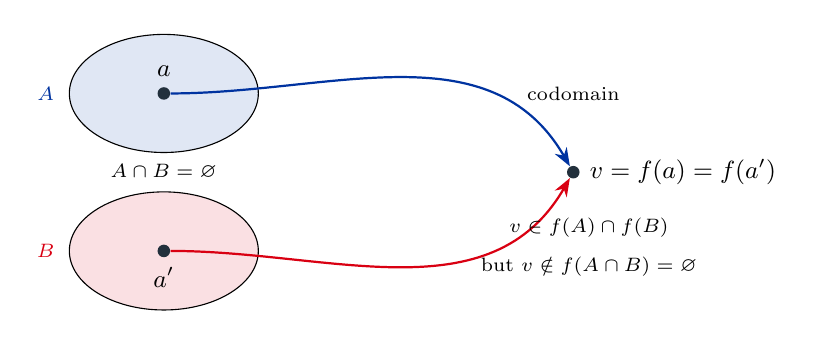
\begin{tikzpicture}[font=\small,>=Stealth, dot/.style={circle,fill=ink,inner sep=1.6pt}]
% set A
\node[draw,ellipse,fill=armBlue!12,minimum width=2.4cm,minimum height=1.5cm] (A) at (0,1.1) {};
\node[font=\scriptsize,armBlue] at (-1.5,1.1) {$A$};
\node[dot,label=above:$a$] (a) at (0,1.1) {};
% set B
\node[draw,ellipse,fill=armRed!12,minimum width=2.4cm,minimum height=1.5cm] (B) at (0,-0.9) {};
\node[font=\scriptsize,armRed] at (-1.5,-0.9) {$B$};
\node[dot,label=below:$a'$] (b) at (0,-0.9) {};
\node[font=\scriptsize] at (0,0.1) {$A\cap B=\varnothing$};
% shared output
\node[dot,label={right:$v=f(a)=f(a')$}] (v) at (5.2,0.1) {};
\node[font=\scriptsize] at (5.2,1.1) {codomain};
\draw[->,armBlue,thick] (a) to[out=0,in=120] (v);
\draw[->,armRed,thick]  (b) to[out=0,in=240] (v);
\node[font=\scriptsize] at (5.4,-0.6) {$v\in f(A)\cap f(B)$};
\node[font=\scriptsize] at (5.4,-1.1) {but $v\notin f(A\cap B)=\varnothing$};
\end{tikzpicture}
\end{center}

\begin{methodbox}
\textbf{Transferable technique:} for image laws, the inclusion that needs no hypothesis is always
\textquotedbl{}image of intersection $\subseteq$ intersection of images.\textquotedbl{} The reverse
needs injectivity, and the counterexample is always two collision points placed in different
singletons. (Union behaves better: $f(A\cup B)=f(A)\cup f(B)$ for \emph{every} $f$.)
\end{methodbox}

% ============================================================================
\section*{Problem 22 - Can disjoint nonempty $X_1,X_2$ have $f(X_1)=f(X_2)$?}

\begin{problembox}[22]
For $f:A\to B$ and disjoint nonempty $X_1,X_2\subseteq A$ (so $X_1\cap X_2=\varnothing$),
\emph{can} the images be equal, $f(X_1)=f(X_2)$?
\end{problembox}

\begin{ideabox}
Images are about \emph{output values}, not about which inputs produced them. Two completely
separate input sets can still hit the very same set of outputs, provided $f$ glues their points
together. So as soon as $f$ is non-injective, the answer is \textbf{yes, equal images are possible}.
(Note the cleanest reading of the question: equal images are not \emph{forced} - take $X_1=\{1\}$,
$X_2=\{2\}$ under the identity to get unequal images - but they \emph{can} happen, which is the
interesting content.)
\end{ideabox}

\textbf{Step 1 - Build an example.} Take $f:\R\to\R$, $f(x)=x^2$, and the disjoint singletons
$X_1=\{1\}$, $X_2=\{-1\}$. They are nonempty and $X_1\cap X_2=\varnothing$.

\textbf{Step 2 - Compute the images.} $f(X_1)=\{1^2\}=\{1\}$ and $f(X_2)=\{(-1)^2\}=\{1\}$. So
$f(X_1)=f(X_2)=\{1\}$, equal images from disjoint sets.

\textbf{Step 3 - Always check the logic.} The trick is exactly non-injectivity: $f$ sends the
distinct points $1$ and $-1$ to the same value. With a larger example, $X_1=\{1,2\}$,
$X_2=\{-1,-2\}$ gives $f(X_1)=\{1,4\}=f(X_2)$ too. (If $f$ \emph{were} injective, disjoint nonempty
sets would always have unequal - indeed disjoint - images.)

\answer{\textbf{Yes}, it is possible. Example: $f(x)=x^2$, $X_1=\{1\}$, $X_2=\{-1\}$ are disjoint
yet $f(X_1)=f(X_2)=\{1\}$. (Equal images are not forced, but they can occur whenever $f$ is not
injective.)}

\medskip
\textbf{Picture: two disjoint sets, one shared image.} The arrow diagram for $f(x)=x^2$ on
$\{-2,-1,1,2\}$: the symmetric pair $\{1,2\}$ and $\{-1,-2\}$ map onto the identical value set
$\{1,4\}$.

\begin{center}
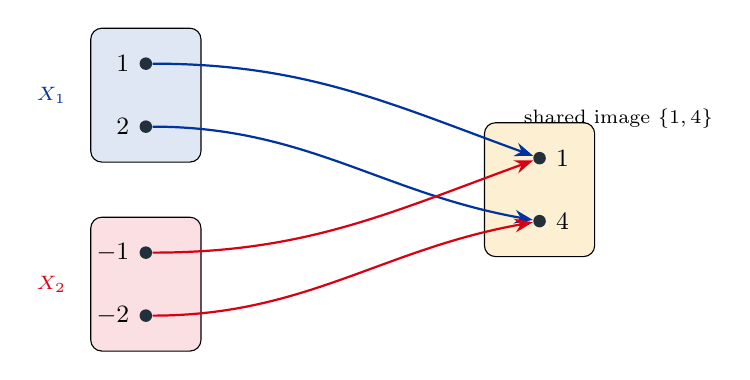
\begin{tikzpicture}[font=\small,>=Stealth, dot/.style={circle,fill=ink,inner sep=1.6pt}]
\node[draw,rounded corners,fill=armBlue!12,minimum width=1.4cm,minimum height=1.7cm] at (0,1.2) {};
\node[font=\scriptsize,armBlue] at (-1.2,1.2) {$X_1$};
\node[dot,label=left:$1$] (p1) at (0,1.6) {};
\node[dot,label=left:$2$] (p2) at (0,0.8) {};
\node[draw,rounded corners,fill=armRed!12,minimum width=1.4cm,minimum height=1.7cm] at (0,-1.2) {};
\node[font=\scriptsize,armRed] at (-1.2,-1.2) {$X_2$};
\node[dot,label=left:$-1$] (m1) at (0,-0.8) {};
\node[dot,label=left:$-2$] (m2) at (0,-1.6) {};
\node[draw,rounded corners,fill=armOrange!18,minimum width=1.4cm,minimum height=1.7cm] at (5,0) {};
\node[font=\scriptsize] at (6.0,0.9) {shared image $\{1,4\}$};
\node[dot,label=right:$1$] (v1) at (5,0.4) {};
\node[dot,label=right:$4$] (v2) at (5,-0.4) {};
\draw[->,armBlue,thick] (p1) to[out=0,in=160] (v1);
\draw[->,armBlue,thick] (p2) to[out=0,in=170] (v2);
\draw[->,armRed,thick]  (m1) to[out=0,in=200] (v1);
\draw[->,armRed,thick]  (m2) to[out=0,in=190] (v2);
\end{tikzpicture}
\end{center}

\begin{methodbox}
\textbf{Transferable technique:} \textquotedbl{}image of a set\textquotedbl{} forgets multiplicity
and origin. Whenever a property is about images alone, a non-injective $f$ (a folding map like
$x^2$ or $|x|$) is your go-to source of surprises.
\end{methodbox}

% ============================================================================
\section*{Problem 24 - Does $Y_1\cap Y_2=\varnothing$ force $f^{-1}(Y_1)\cap f^{-1}(Y_2)=\varnothing$?}

\begin{problembox}[24]
Is it correct that for $f:A\to B$ and $Y_1,Y_2\subseteq B$, if $Y_1\cap Y_2=\varnothing$ then
$f^{-1}(Y_1)\cap f^{-1}(Y_2)=\varnothing$?
\end{problembox}

\begin{ideabox}
Preimages behave \emph{perfectly} - much better than images - because each input $x$ has exactly
\emph{one} output $f(x)$, so asking \textquotedbl{}is $x$ in $f^{-1}(Y)$?\textquotedbl{} is just
asking \textquotedbl{}is the single value $f(x)$ in $Y$?\textquotedbl{} If $x$ were in both
preimages, the one value $f(x)$ would have to live in both $Y_1$ and $Y_2$ at once - impossible
when they are disjoint. No injectivity needed; this is \textbf{always} true. The deeper fact is
$f^{-1}(Y_1)\cap f^{-1}(Y_2)=f^{-1}(Y_1\cap Y_2)$ for every $f$.
\end{ideabox}

\textbf{Step 1 - Suppose the intersection is nonempty and derive a contradiction.} Let
$x\in f^{-1}(Y_1)\cap f^{-1}(Y_2)$. Then $f(x)\in Y_1$ and $f(x)\in Y_2$, so
$f(x)\in Y_1\cap Y_2$.

\textbf{Step 2 - Use disjointness.} But $Y_1\cap Y_2=\varnothing$, so $f(x)$ belongs to the empty
set - impossible. Hence no such $x$ exists, and $f^{-1}(Y_1)\cap f^{-1}(Y_2)=\varnothing$.

\textbf{Step 3 - The clean reason (general identity).} For any $x$:
\[
x\in f^{-1}(Y_1)\cap f^{-1}(Y_2)
\iff f(x)\in Y_1 \text{ and } f(x)\in Y_2
\iff f(x)\in Y_1\cap Y_2
\iff x\in f^{-1}(Y_1\cap Y_2).
\]
So $f^{-1}(Y_1)\cap f^{-1}(Y_2)=f^{-1}(Y_1\cap Y_2)$ \emph{always}, and the disjoint case is the
special instance $Y_1\cap Y_2=\varnothing\Rightarrow f^{-1}(\varnothing)=\varnothing$.

\textbf{Step 4 - Always check on a concrete map.} Step 3 proves the identity for every $f$; a
concrete instance with $f(x)=x^2$ ($Y_1=\{1\}$, $Y_2=\{4\}$ giving disjoint preimages
$\{\pm1\},\{\pm2\}$, whose union is $f^{-1}(\{1,4\})$) bears out both the identity
$f^{-1}(Y_1)\cap f^{-1}(Y_2)=f^{-1}(Y_1\cap Y_2)$ and the disjoint consequence.

\answer{\textbf{Yes, always} (no hypothesis on $f$ needed). Indeed
$f^{-1}(Y_1)\cap f^{-1}(Y_2)=f^{-1}(Y_1\cap Y_2)$, so disjoint $Y$'s give disjoint preimages.}

\medskip
\textbf{Why preimages cannot overlap here.} Each input has a single output, so it can only sit in
the preimage of whichever target block contains that one value. Disjoint target blocks $\Rightarrow$
each input is committed to at most one $\Rightarrow$ no input is shared.

\begin{center}
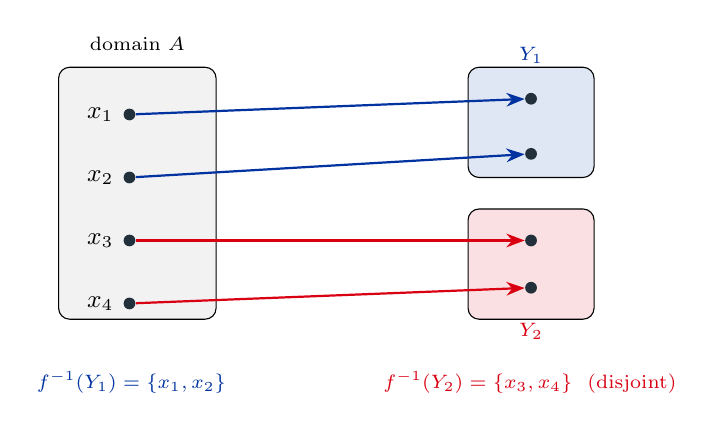
\begin{tikzpicture}[font=\small,>=Stealth, dot/.style={circle,fill=ink,inner sep=1.5pt}]
% domain
\node[draw,rounded corners,fill=gray!10,minimum width=2cm,minimum height=3.2cm] at (0,0) {};
\node[font=\scriptsize] at (0,1.9) {domain $A$};
\node[dot,label=left:$x_1$] (x1) at (-0.1,1.0) {};
\node[dot,label=left:$x_2$] (x2) at (-0.1,0.2) {};
\node[dot,label=left:$x_3$] (x3) at (-0.1,-0.6) {};
\node[dot,label=left:$x_4$] (x4) at (-0.1,-1.4) {};
% codomain with two disjoint blocks
\node[draw,rounded corners,fill=armBlue!12,minimum width=1.6cm,minimum height=1.4cm] at (5,0.9) {};
\node[font=\scriptsize,armBlue] at (5,1.75) {$Y_1$};
\node[draw,rounded corners,fill=armRed!12,minimum width=1.6cm,minimum height=1.4cm] at (5,-0.9) {};
\node[font=\scriptsize,armRed] at (5,-1.75) {$Y_2$};
\node[dot] (u1) at (5,1.2) {};
\node[dot] (u2) at (5,0.5) {};
\node[dot] (u3) at (5,-0.6) {};
\node[dot] (u4) at (5,-1.2) {};
\draw[->,armBlue,thick] (x1) -- (u1);
\draw[->,armBlue,thick] (x2) -- (u2);
\draw[->,armRed,thick]  (x3) -- (u3);
\draw[->,armRed,thick]  (x4) -- (u4);
\node[font=\scriptsize,armBlue,anchor=west] at (-1.4,-2.4) {$f^{-1}(Y_1)=\{x_1,x_2\}$};
\node[font=\scriptsize,armRed,anchor=west]  at (3.0,-2.4) {$f^{-1}(Y_2)=\{x_3,x_4\}$ \ (disjoint)};
\end{tikzpicture}
\end{center}

\begin{methodbox}
\textbf{Transferable technique:} preimage commutes with \emph{everything} - intersection, union,
and complement - for \emph{every} function: $f^{-1}(Y_1\cap Y_2)=f^{-1}(Y_1)\cap f^{-1}(Y_2)$,
similarly for $\cup$ and complement. This is because a preimage is defined by a single membership
test on the one value $f(x)$. Images are the badly behaved direction; preimages are the friendly
one.
\end{methodbox}

% ============================================================================
\section*{Problem 25 - $f(f^{-1}(Y))\subseteq Y$, with a strict example}

\begin{problembox}[25]
Show that $f(f^{-1}(Y))\subseteq Y$ for every $f:A\to B$ and $Y\subseteq B$. Give an example where
the inclusion is strict.
\end{problembox}

\begin{ideabox}
Read the two operations literally. The preimage $f^{-1}(Y)$ is \textquotedbl{}all inputs whose
output lands in $Y$.\textquotedbl{} Apply $f$ to that set and you get back outputs that, by
construction, were already in $Y$. So you can only land back inside $Y$ - never escape it. Why
might you not fill all of $Y$? Because $Y$ may contain target values that $f$ \emph{never produces}
(values outside the range). Those have no inputs pointing at them, so $f(f^{-1}(Y))$ misses them,
making the inclusion strict.
\end{ideabox}

\textbf{Step 1 - Prove the inclusion.} Let $y\in f(f^{-1}(Y))$. Then $y=f(x)$ for some
$x\in f^{-1}(Y)$. But $x\in f^{-1}(Y)$ means exactly that $f(x)\in Y$. So $y=f(x)\in Y$. As $y$ was
arbitrary, $f(f^{-1}(Y))\subseteq Y$.

\textbf{Step 2 - Build a strict example.} Take $f:\R\to\R$, $f(x)=x^2$, and $Y=\{-1,1\}$. Then
\[
f^{-1}(Y)=\{x:x^2\in\{-1,1\}\}=\{x:x^2=1\}=\{-1,1\}
\]
(no real $x$ has $x^2=-1$), and applying $f$:
\[
f\bigl(\{-1,1\}\bigr)=\{1\}.
\]
So $f(f^{-1}(Y))=\{1\}\subsetneq\{-1,1\}=Y$. The value $-1\in Y$ is outside the range of $f$, so it
is dropped.

\textbf{Step 3 - Always check the boundary condition.} Equality $f(f^{-1}(Y))=Y$ holds exactly when
$Y\subseteq f(A)$ (every element of $Y$ is actually produced). Here $-1\notin f(\R)=[0,\infty)$, so
strictness is forced. Step 1 already proves $f(f^{-1}(Y))\subseteq Y$ for every $f$; the example
above is a concrete instance of the strict drop.

\answer{$f(f^{-1}(Y))\subseteq Y$ always. Strict example: $f(x)=x^2$, $Y=\{-1,1\}$ gives
$f(f^{-1}(Y))=\{1\}\subsetneq Y$ (the value $-1$ is never an output).}

\medskip
\textbf{Picture: the unreachable target gets dropped.} Pull $Y=\{-1,1\}$ back to its preimage, then
push forward. Only $1$ survives, because $-1$ has no arrow coming into it.

\begin{center}
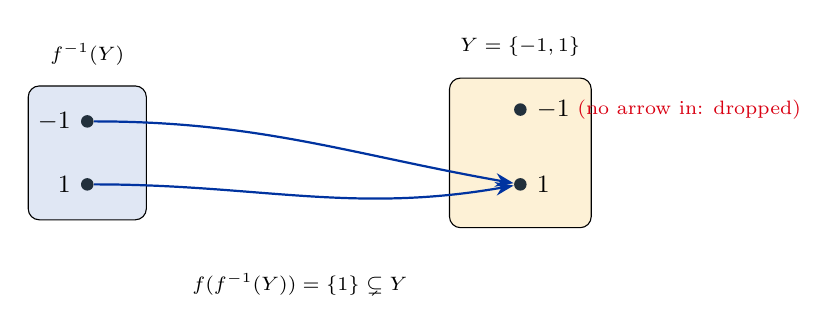
\begin{tikzpicture}[font=\small,>=Stealth, dot/.style={circle,fill=ink,inner sep=1.6pt}]
% domain : preimage
\node[draw,rounded corners,fill=armBlue!12,minimum width=1.5cm,minimum height=1.7cm] at (0,0) {};
\node[font=\scriptsize] at (0,1.25) {$f^{-1}(Y)$};
\node[dot,label=left:$-1$] (n) at (0,0.4) {};
\node[dot,label=left:$1$]  (p) at (0,-0.4) {};
% codomain : Y with one unreachable point
\node[draw,rounded corners,fill=armOrange!16,minimum width=1.8cm,minimum height=1.9cm] at (5.5,0) {};
\node[font=\scriptsize] at (5.5,1.35) {$Y=\{-1,1\}$};
\node[dot,label=right:$1$]  (y1) at (5.5,-0.4) {};
\node[dot,label=right:$-1$] (ym) at (5.5,0.55) {};
\node[font=\scriptsize,armRed,anchor=west] at (6.1,0.55) {(no arrow in: dropped)};
\draw[->,armBlue,thick] (n) to[out=0,in=170] (y1);
\draw[->,armBlue,thick] (p) to[out=0,in=190] (y1);
\node[font=\scriptsize,anchor=north] at (2.7,-1.4) {$f(f^{-1}(Y))=\{1\}\subsetneq Y$};
\end{tikzpicture}
\end{center}

\begin{methodbox}
\textbf{Transferable technique:} the two round trips go opposite ways. Pushing then pulling
\emph{shrinks or stays}: $f(f^{-1}(Y))\subseteq Y$ (equality iff $Y\subseteq f(A)$). Pulling then
pushing \emph{grows or stays}: $X\subseteq f^{-1}(f(X))$ (equality iff $f$ is injective). Memorize
the direction of each $\subseteq$ by asking \textquotedbl{}can a value/point be lost or
gained?\textquotedbl{}
\end{methodbox}

\end{document}
